\section{Two campaigns: 25B + 30B tokens}
\label{sec:vision-campaigns}

\begin{figure}[t]
\centering
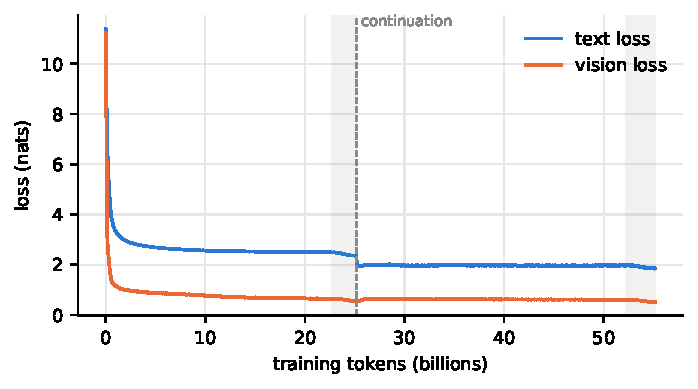
\includegraphics[width=0.94\linewidth]{figures/vision_loss_curves.pdf}
\caption{Vision and text loss across both campaigns on one cumulative
axis (EMA-smoothed). Shaded spans are the two terminal anneals; the
dashed line marks the warm-start into the continuation, whose re-warmed
learning rate briefly gives back the first anneal's polish.}
\label{fig:vision-loss}
\end{figure}

\textbf{Trial (48{,}000 steps, 25.2B tokens).} From-scratch joint
training at sequence length 4096, per-device batch 4 (524{,}288
tokens/step), MuonClip at LR $1.2\times10^{-3}$, terminal cosine anneal
over the final 4{,}800 steps. The tower's output scale told the run's
most instructive story (Figure~\ref{fig:embed-ratio}): unconstrained by
any output norm, the visual/text embedding RMS ratio overshot from 0.60
to 4.98 by step 5k, then declined monotonically as the loss pulled the
tower onto the language manifold --- no intervention required, which is
precisely what the probe was built to establish.

\begin{figure}[t]
\centering
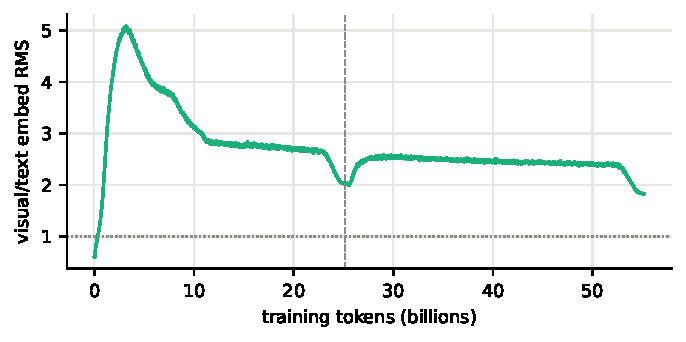
\includegraphics[width=0.94\linewidth]{figures/embed_ratio.pdf}
\caption{Post-splice visual/text embedding RMS ratio. The from-scratch
tower overshoots the language scale $5\times$ early, then
self-regulates; each anneal pulls it further toward parity.}
\label{fig:embed-ratio}
\end{figure}

\textbf{Continuation (57{,}220 steps, 30.0B tokens).} Warm-started from
the trial's annealed checkpoint with a fresh optimizer and a 1{,}500-step
re-warmup, adding the code and mathematics streams of
Section~\ref{sec:vision-data}. One observation deserves record: through
the continuation's terminal anneal the \emph{pure web-text} holdout
degraded by $\sim$0.1 nats while the training mixture kept improving
--- as the learning rate vanishes the model converges precisely to the
\emph{mixture} optimum, exposing its distance from the pure-text
optimum. Convergence reveals allocation; the capability sections show
what the reallocation bought.

\textbf{Stability.} Across 105{,}220 steps and 55B tokens: zero
non-finite losses or gradients, zero QK-clip activations, and --- the
gate's validation --- cycle-0 attention max-logits alive in the 8--14
band throughout, including the step-30k--40k window where Part~I's
ungated campaign collapsed permanently to zero. Gradient norms stayed
in the 0.04--0.14 band with the tower's share rising $15\times$ as
visual features became load-bearing.

\textbf{Operations.} Each campaign survived one mid-run failure
(a hung parquet read without a timeout; a closed HTTP client), both
recovered by weights-and-optimizer resume from 4{,}000-step per-host
local checkpoints with the stream restarting --- the streaming
checkpoint policy of Part~I unchanged. Both root causes were then
eliminated in code (timeouts; the self-healing draw), not in runbooks.
